%==============================================================================
% Appendix Figures
%==============================================================================

%------------------------------------------------------------------------------
% Figure A.1: All four experiment conditions
%------------------------------------------------------------------------------
\begin{figure}[htbp]
\caption{Experiment conditions}
\centering
\setlength{\fboxsep}{3pt}
\setlength{\fboxrule}{0.6pt}
\begin{tabular}{cc}
\fbox{
\includegraphics[width=0.46\textwidth]{../slides/control.png}} &
\fbox{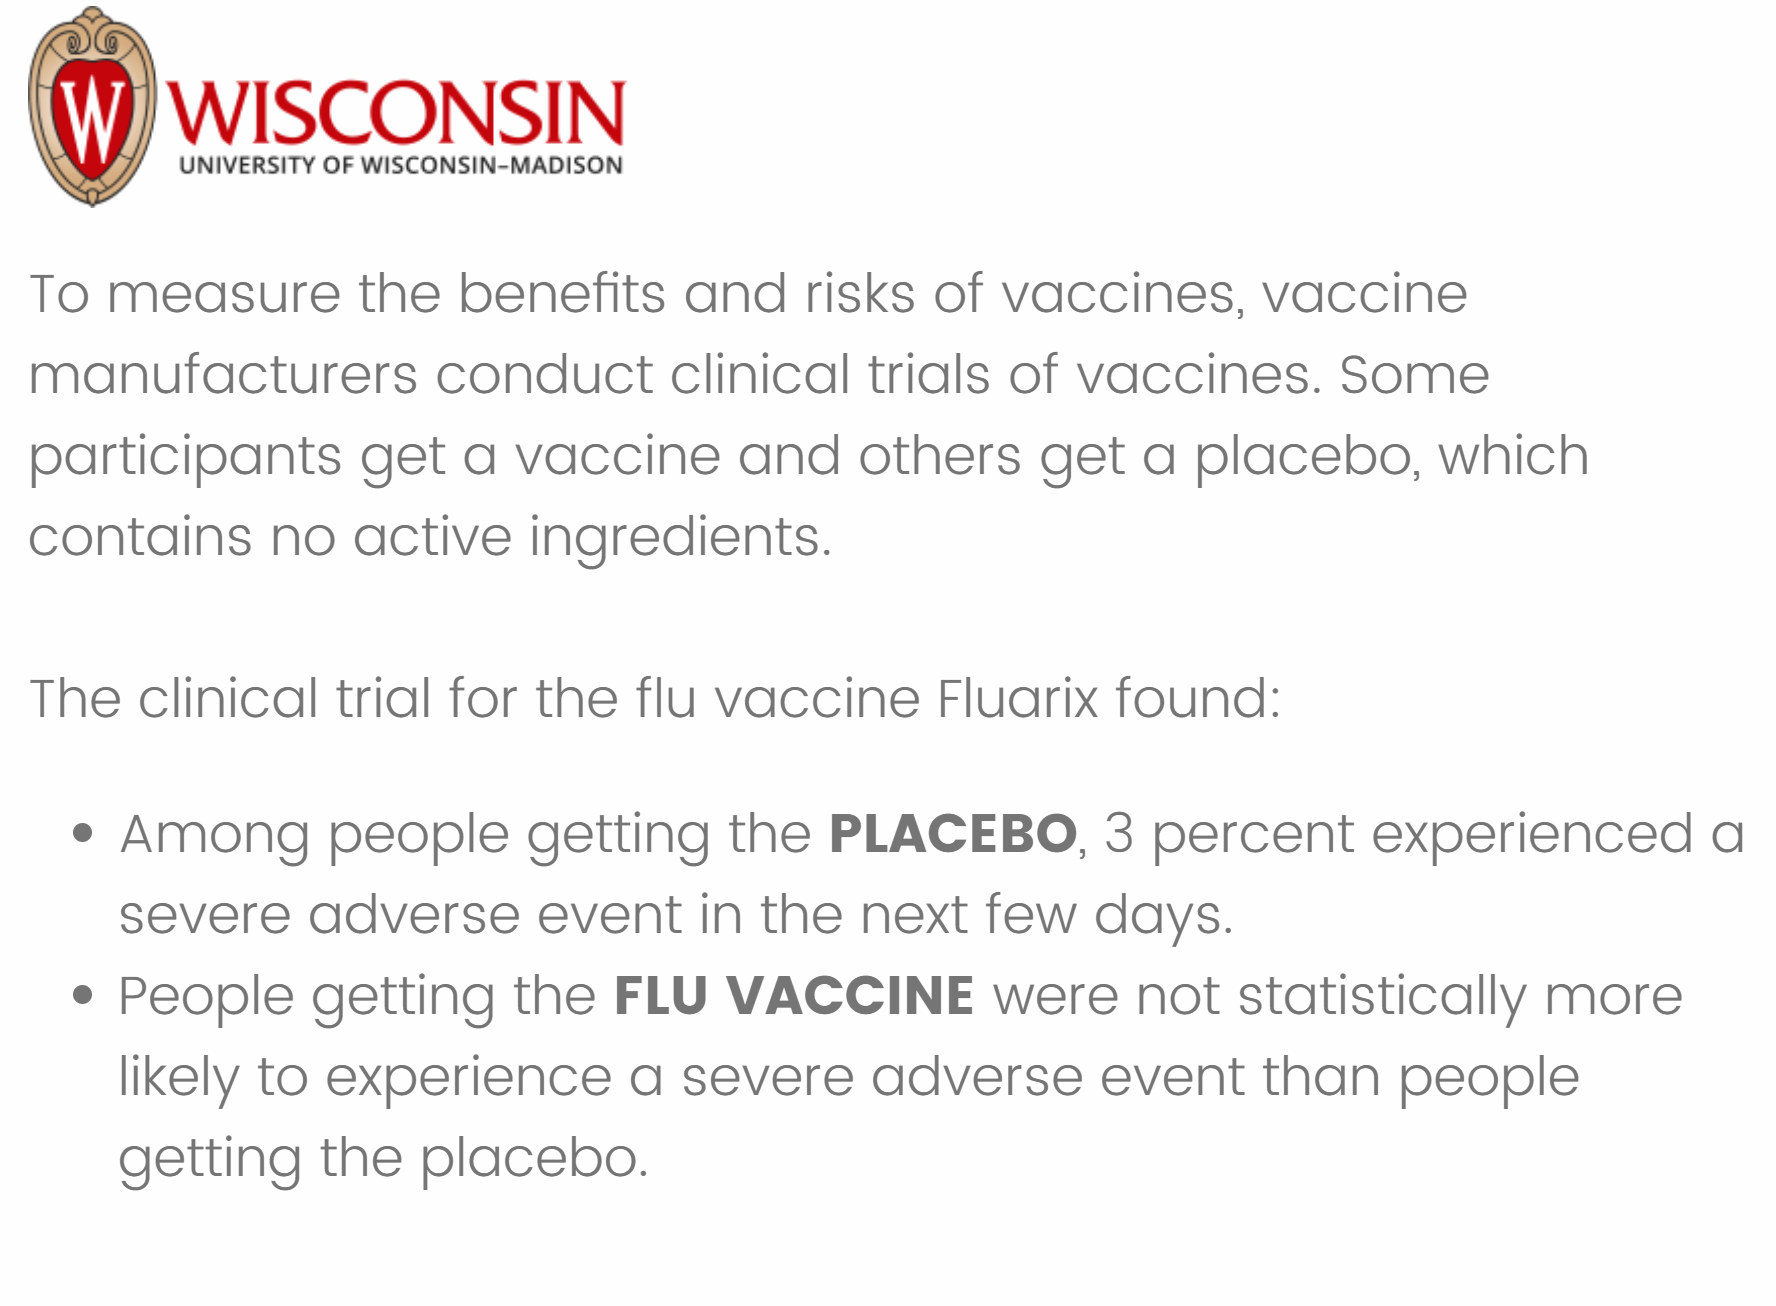
\includegraphics[width=0.46\textwidth]{../slides/industry.png}} \\[4pt]
(a) Control & (b) Industry \\[14pt]
\fbox{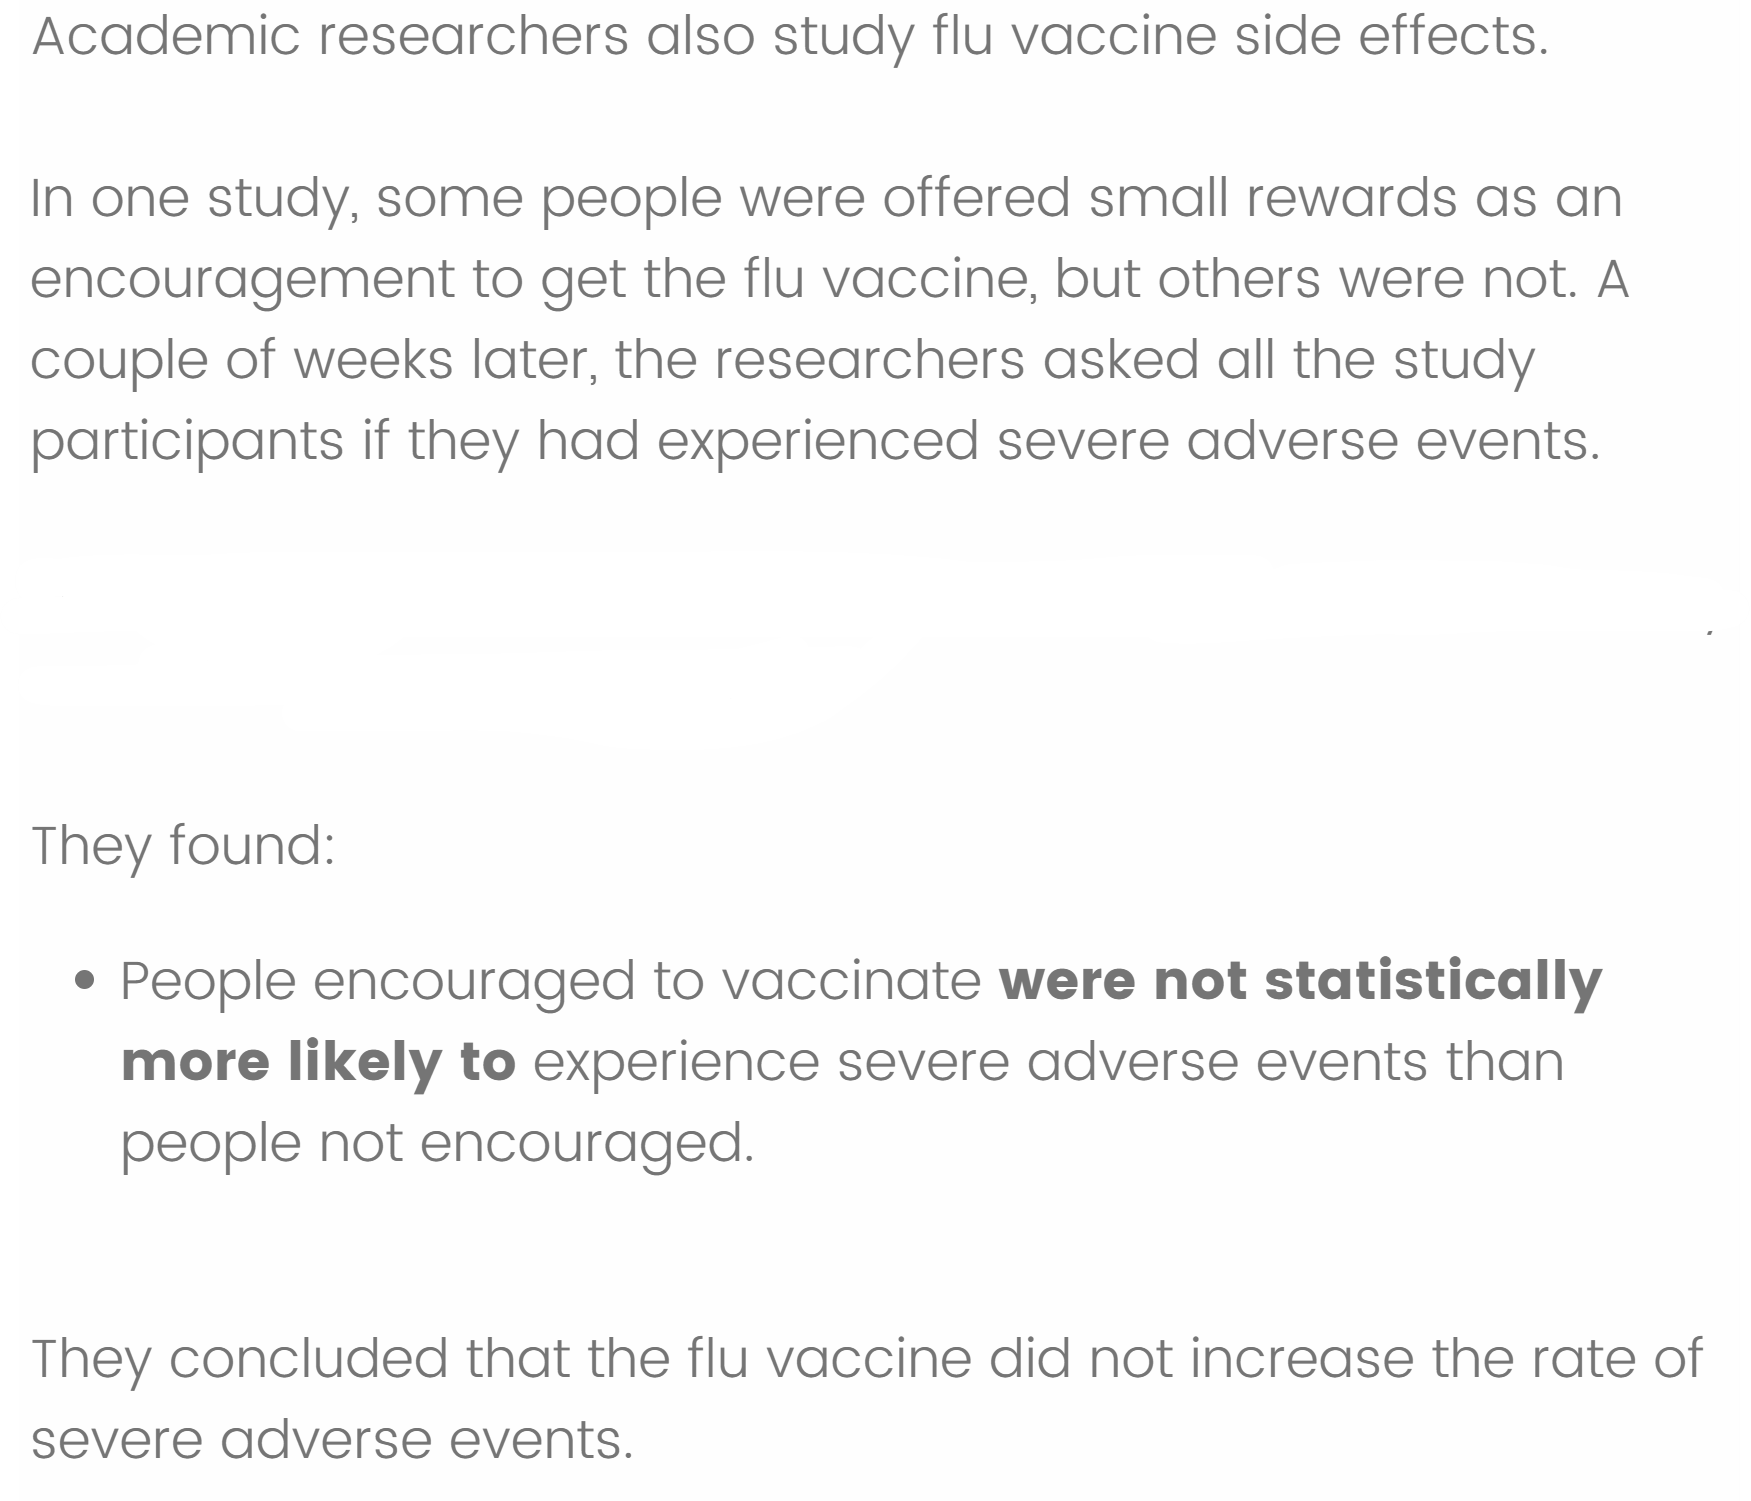
\includegraphics[width=0.46\textwidth]{../slides/academic.png}} &
\fbox{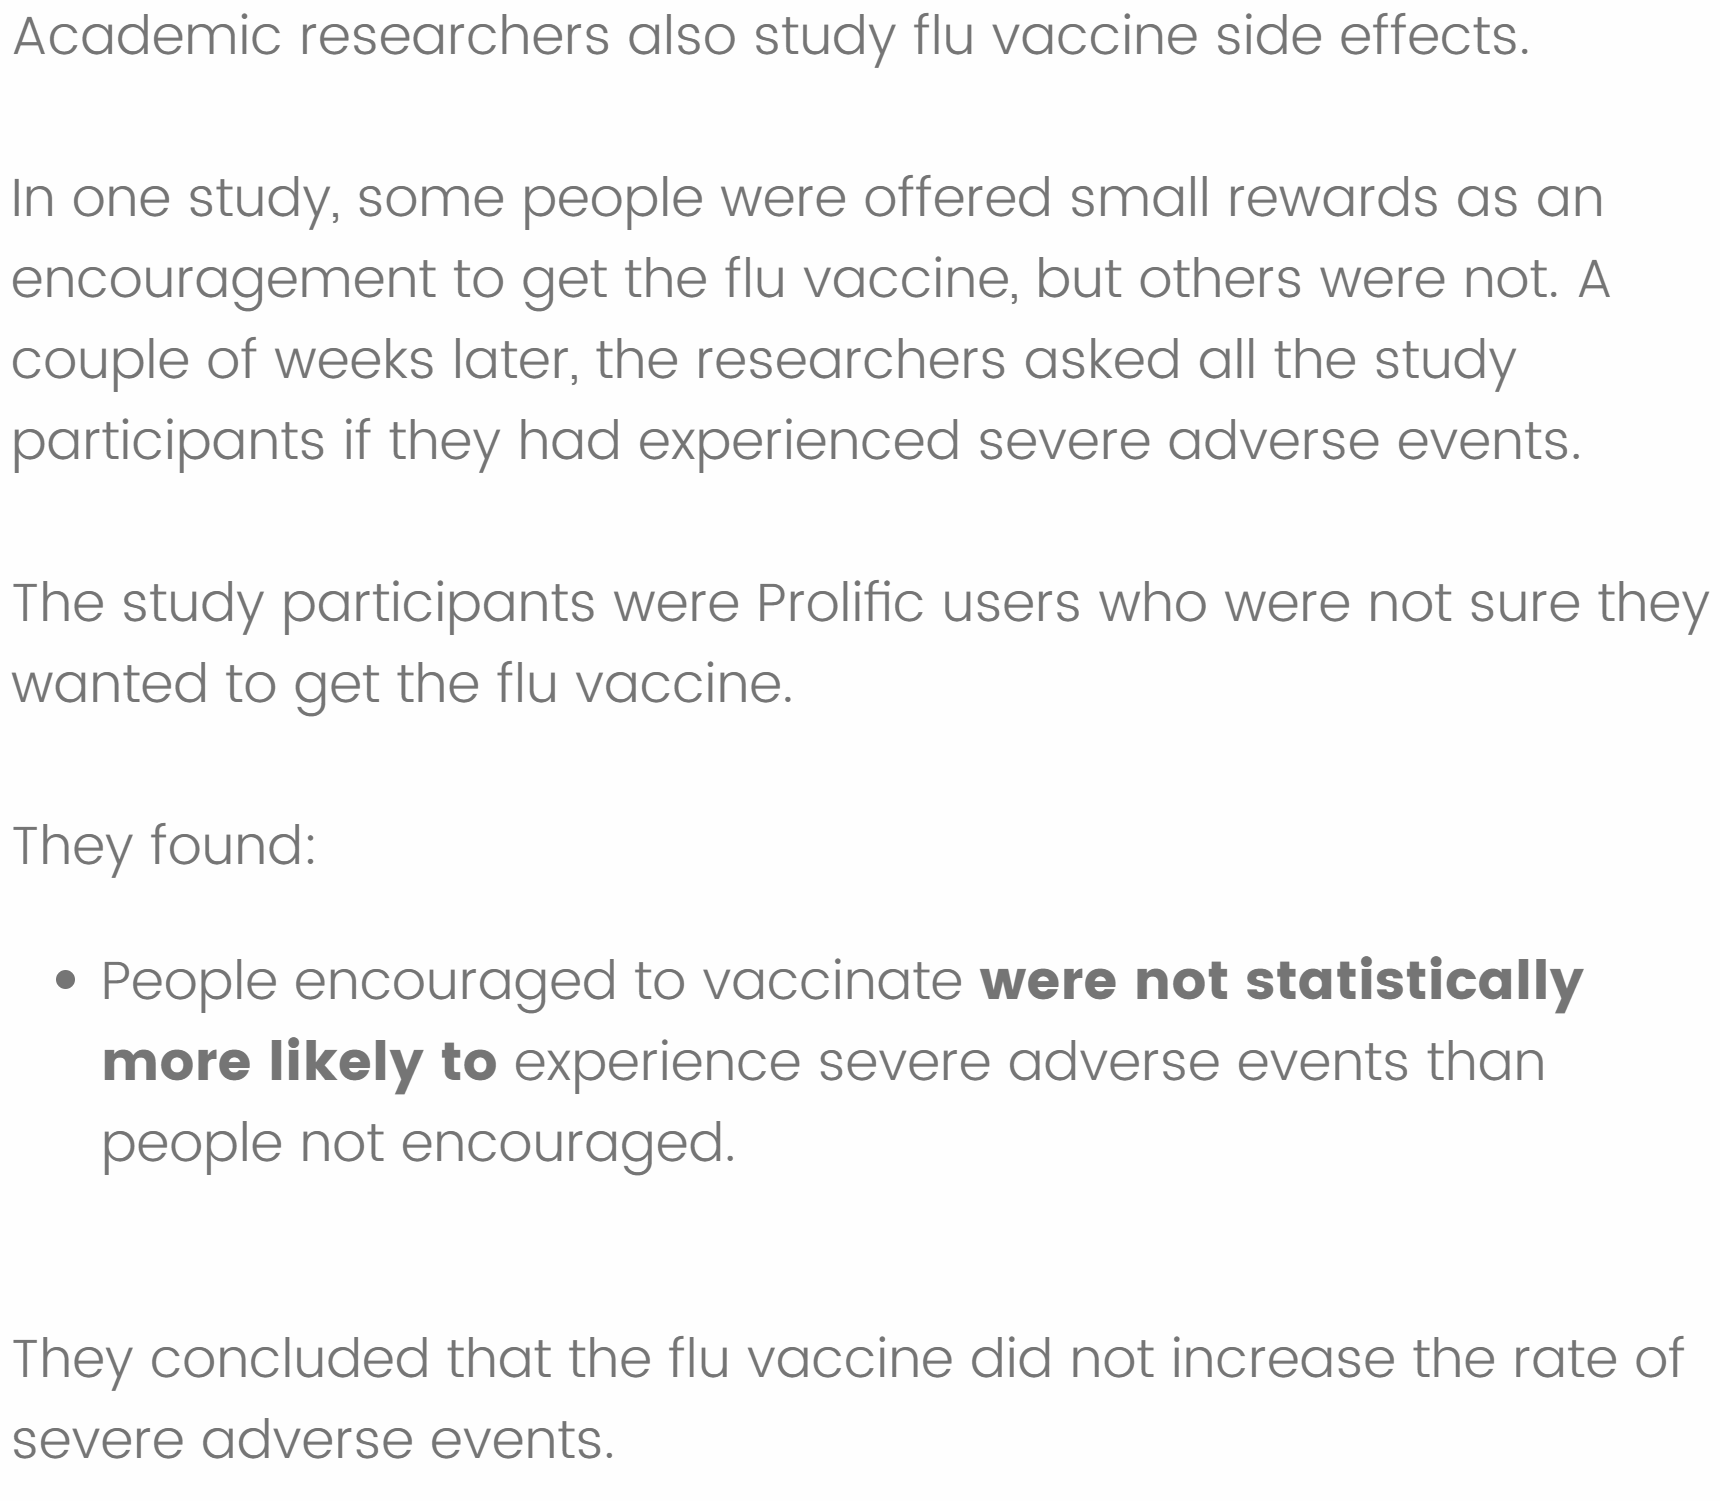
\includegraphics[width=0.46\textwidth]{../slides/personal.png}} \\[4pt]
(c) Academic (additional info beyond control) & (d) Representative  (additional info) 
beyond controls\\
\end{tabular}
\label{fig:interventions}
\fignote{\linewidth}{Screenshots of the information screens for all four
treatment arms. Participants in the academic and representative arms saw 
the control arm information as well as the information about the academic study.}
\end{figure}



\begin{figure}
\caption{Trust in government and following doctor's advice by vaccine hesitancy}
\label{fig:trust_by_hes}
\centering 
\includegraphics[height=0.8\textheight]{../output/figures/trust_by_hes.png}
\fignote{\linewidth}{Notes: Top panel reports s the fraction of vaccine hesitant
and non-hesitant participants who report using the indicated source "sometimes"
or "often" for health care information. Bottom panel reports the fraction 
who view the source as "reliable" (as opposed to "somewhat reliable" or "not reliable"),
conditional on using that source. }
\end{figure}